\chapter{Fungsi}

\section*{Pengantar}

Konsep fungsi merupakan fondasi utama dalam matematika rekayasa. Dalam Bab~1, kita telah mempelajari persamaan garis lurus yang merupakan contoh sederhana dari fungsi linear. Pada bab ini, konsep tersebut diperluas ke fungsi yang lebih umum, termasuk fungsi kuadrat, trigonometri, eksponensial, dan logaritmik. Pemahaman tentang sifat-sifat fungsi (daerah definisi, genap-ganjil, periodik, monoton) menjadi landasan penting untuk topik-topik selanjutnya, khususnya \textbf{pendekatan akar} (Bab~3) yang mencari titik-titik nol $f(x) = 0$ secara numerik, \textbf{interpolasi} (Bab~4) yang pada dasarnya adalah pendekatan fungsi dari data diskrit, \textbf{integral kalkulus} (Bab~5) yang menghitung luasan di bawah kurva fungsi, serta \textbf{Deret Fourier} (Bab~6) yang merepresentasikan fungsi periodik sebagai superposisi sinusoidal.

\section{Definisi Fungsi}

Diberikan $y = f(x)$, dibaca ``$y$ adalah fungsi dari $x$.'' Variabel $x$ disebut \textbf{peubah bebas} dan $y$ disebut \textbf{peubah tak bebas}. $y$ dikatakan sebagai fungsi $x$ jika \textit{setiap satu harga $x$ menentukan tepat satu harga $y$}.

Sebagai contoh: $y = x^2$ merupakan fungsi karena setiap nilai $x$ menghasilkan tepat satu nilai $y$. Sebaliknya, $y^2 = x$ \textbf{bukan} fungsi $x$ karena satu nilai $x$ dapat menghasilkan dua nilai $y$ (misalnya $x = 4$ memberikan $y = 2$ dan $y = -2$).

\begin{figure}[!h]
\centering
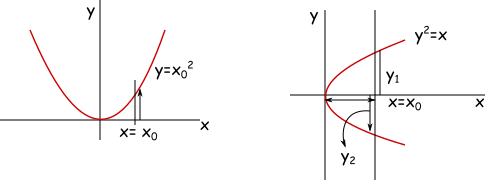
\includegraphics[width=4in]{pict/fungsi1}
\caption{Uji garis vertikal: grafik $y = x^2$ (kiri) lolos uji dan merupakan fungsi; grafik $y^2 = x$ (kanan) tidak lolos uji.}\label{fig:fungsi1}
\end{figure}

\section{Daerah Definisi dan Daerah Fungsi}

\textbf{Daerah definisi} (\textit{domain}) adalah himpunan semua nilai $x$ yang dapat menghasilkan nilai $y$ terdefinisi. \textbf{Daerah fungsi} (\textit{range}) adalah himpunan semua nilai $y$ yang dapat dihasilkan dari daerah definisi.

\begin{exmp}
Tentukan daerah definisi dan daerah fungsi dari fungsi-fungsi berikut!

\begin{enumerate}[(a)]
\item $y = 4x^2$: domain $(-\infty, \infty)$, range $[0, \infty)$.
\item $y = 2x^2 + 1$: domain $(-\infty, \infty)$, range $[1, \infty)$.
\item $y = x^2 - 4$: domain $(-\infty, \infty)$, range $[-4, \infty)$.
\item $y = \sqrt{9 - x^2}$: domain $[-3, 3]$, range $[0, 3]$.
\item $y = \log_2 x$: domain $(0, \infty)$, range $(-\infty, \infty)$.
\item $y = 2\sin(3x)$: domain $(-\infty, \infty)$, range $[-2, 2]$.
\end{enumerate}
\end{exmp}

\section{Macam-macam Fungsi}

\subsection{Berdasarkan Banyaknya Peubah Bebas}
\begin{enumerate}
\item $y = 2x + 1 \longrightarrow$ fungsi 1 peubah.
\item $F(x,y) = x + 2y + 5 \longrightarrow$ fungsi 2 peubah.
\item $F = x^2 + y^2 + z^2 \longrightarrow$ fungsi 3 peubah.
\end{enumerate}

\subsection{Berdasarkan Cara Penyajian}

\begin{enumerate}
\item \textbf{Fungsi eksplisit}: $x$ dan $y$ ditulis dalam ruas yang terpisah, misalnya $y = x^2 + x - 5$.
\item \textbf{Fungsi implisit}: $x$ dan $y$ ditulis dalam ruas yang sama, dilambangkan $f(x,y) = 0$. Contoh: $x^2 + y - 10 = 0$.
\item \textbf{Fungsi parametrik}: $x$ dan $y$ dinyatakan melalui parameter $t$:
\[
x = 10 + t, \quad y = 2t^2 + 4t.
\]
\end{enumerate}

\section{Jenis-jenis Fungsi}

\subsection{Fungsi Aljabar}

$y$ disebut fungsi aljabar dari $x$ jika $y$ diperoleh melalui operasi aljabar berhingga (penjumlahan, pengurangan, perkalian, pembagian, dan penarikan akar) terhadap $x$. Contoh:
\begin{itemize}
\item $y = \dfrac{x+2}{x+1}$ : fungsi aljabar pecahan rasional.
\item $y = \sqrt{x+4}$ : fungsi aljabar irasional.
\end{itemize}

\subsection{Fungsi Transenden}

Fungsi yang \textbf{bukan} fungsi aljabar disebut fungsi transenden. Jenis-jenisnya antara lain:
\begin{itemize}
\item \textbf{Fungsi eksponensial}: $y = a^x$, dengan $a > 0$, $a \ne 1$.
\item \textbf{Fungsi logaritmik}: $y = \log_a x$, dengan $a > 0$, $a \ne 1$.
\item \textbf{Fungsi trigonometri}: $y = \sin x$, $y = \cos x$, $y = \tan x$, dsb.
\item \textbf{Fungsi hiperbolik}: $y = \sinh x = \dfrac{e^x - e^{-x}}{2}$.
\item \textbf{Fungsi siklometri} (invers trigonometri): $y = \arcsin x$, $y = \arccos x$, dsb.
\end{itemize}

\subsection{Fungsi Genap dan Fungsi Ganjil}

Fungsi $f(x)$ dikatakan \textbf{genap} jika $f(-x) = f(x)$ untuk semua $x$ dalam domainnya. Secara geometris, grafiknya simetris terhadap sumbu $y$.

Fungsi $f(x)$ dikatakan \textbf{ganjil} (gasal) jika $f(-x) = -f(x)$. Secara geometris, grafiknya simetris terhadap titik asal $(0,0)$.

\begin{exmp}
Tentukan apakah fungsi-fungsi berikut genap, ganjil, atau tidak keduanya!
\begin{enumerate}[(a)]
\item $f(x) = \cos(x)$: karena $\cos(-x) = \cos(x)$, maka $f$ adalah fungsi \textbf{genap}.
\item $f(x) = \sin(x)$: karena $\sin(-x) = -\sin(x)$, maka $f$ adalah fungsi \textbf{ganjil}.
\item $f(x) = x^2 + 2$: karena $f(-x) = (-x)^2 + 2 = x^2 + 2 = f(x)$, maka $f$ adalah fungsi \textbf{genap}.
\item $f(x) = x^2 + x$: karena $f(-x) = x^2 - x \ne f(x)$ dan $f(-x) \ne -f(x)$, maka $f$ \textbf{bukan genap maupun ganjil}.
\end{enumerate}
\end{exmp}

Sifat genap dan ganjil dari fungsi ini sangat penting dalam analisis \textbf{Deret Fourier} (Bab~6). Jika fungsi periodik bersifat genap, maka koefisien sinus $b_n = 0$ (deret hanya mengandung kosinus), dan jika ganjil, maka koefisien kosinus $a_n = 0$ (deret hanya mengandung sinus).

\subsection{Fungsi Periodik}

Fungsi $f(x)$ dikatakan \textbf{periodik} dengan periode $T$ jika
\[
f(x + T) = f(x)
\]
untuk semua $x$ dalam domainnya, dan $T$ adalah bilangan positif terkecil yang memenuhi syarat tersebut.

\begin{exmp}
Tentukan periode dari fungsi-fungsi berikut!
\begin{enumerate}[(a)]
\item $y = 2\sin(3x)$: periode $T = 2\pi/3$.
\item $y = 4\tan(2x)$: periode $T = \pi/2$.
\item $y = 4\cos\!\left(6x + \frac{\pi}{3}\right)$: periode $T = 2\pi/6 = \pi/3$.
\end{enumerate}
\end{exmp}

Fungsi periodik akan dibahas secara mendalam pada Bab~6 (Deret Fourier) dan Bab~7 (Analisa Sistem), di mana sinyal-sinyal periodik direpresentasikan sebagai penjumlahan komponen sinusoidal.

\subsection{Fungsi Homogen}

Fungsi $f(x,y)$ disebut \textbf{homogen berderajat $n$} jika
\[
f(\lambda x,\, \lambda y) = \lambda^n\, f(x,y)
\]
untuk sebarang $\lambda$.

\begin{exmp}
Tentukan derajat kehomogenan fungsi-fungsi berikut!
\begin{enumerate}[(a)]
\item $f(x,y) = \sqrt[3]{x^3 + y^3}$: karena $f(\lambda x, \lambda y) = \sqrt[3]{\lambda^3 x^3 + \lambda^3 y^3} = \lambda\,\sqrt[3]{x^3+y^3} = \lambda\,f(x,y)$, maka homogen berderajat \textbf{1}.
\item $f(x,y) = 2xy - y^2$: karena $f(\lambda x, \lambda y) = 2\lambda^2 xy - \lambda^2 y^2 = \lambda^2 f(x,y)$, maka homogen berderajat \textbf{2}.
\item $f(x,y) = xy^3 - x^3 y$: karena $f(\lambda x, \lambda y) = \lambda^4(xy^3 - x^3 y) = \lambda^4 f(x,y)$, maka homogen berderajat \textbf{4}.
\end{enumerate}
\end{exmp}

\subsection{Fungsi Naik dan Fungsi Turun}

Fungsi $f(x)$ disebut \textbf{fungsi naik} pada interval $I$ jika $f'(x) > 0$ untuk semua $x \in I$, dan \textbf{fungsi turun} jika $f'(x) < 0$.

\begin{exmp}
Tentukan interval fungsi naik dan turun dari $y = x^2 - 2x + 3$!

\textbf{Penyelesaian:}\\
$y' = 2x - 2 = 0 \Rightarrow x = 1$.
\begin{itemize}
\item Untuk $x < 1$: $y' < 0$, fungsi \textbf{turun}.
\item Untuk $x > 1$: $y' > 0$, fungsi \textbf{naik}.
\end{itemize}
Titik minimum terjadi di $x = 1$ dengan $y_{\min} = 2$.
\end{exmp}

\begin{exmp}
Tentukan interval fungsi naik dan turun dari $y = 2x^3 - 3x^2 - 36x + 4$!

\textbf{Penyelesaian:}\\
$y' = 6x^2 - 6x - 36 = 6(x^2 - x - 6) = 6(x-3)(x+2) = 0 \Rightarrow x = 3$ atau $x = -2$.
\begin{itemize}
\item Untuk $x < -2$: $y' > 0$, fungsi \textbf{naik}.
\item Untuk $-2 < x < 3$: $y' < 0$, fungsi \textbf{turun}.
\item Untuk $x > 3$: $y' > 0$, fungsi \textbf{naik}.
\end{itemize}
\end{exmp}

\subsection{Fungsi Invers}

Fungsi invers $f^{-1}(x)$ diperoleh dengan mencerminkan seluruh titik fungsi $f(x)$ terhadap garis $y = x$. Secara praktis, fungsi invers diperoleh dengan \textbf{menukar $x$ dan $y$} pada persamaan $y = f(x)$ kemudian menyatakan $y$ sebagai fungsi $x$.

\begin{figure}[!h]
\centering
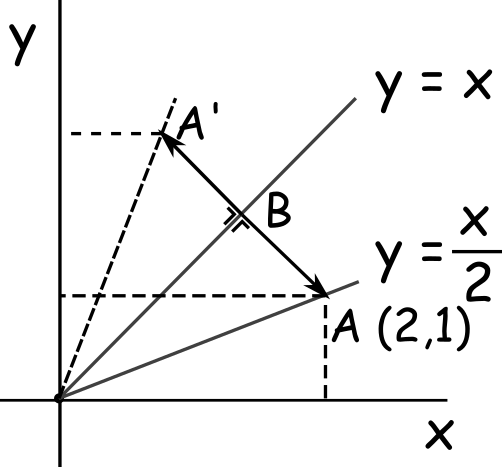
\includegraphics[width=1.5in]{pict/fungsiInvers}
\caption{Pencerminan $y = x/2$ terhadap garis $y = x$ menghasilkan $y = 2x$.}\label{fig:fungsiInvers}
\end{figure}

\begin{exmp}
Tentukan invers dari fungsi $f(x) = x/2$!

\textbf{Penyelesaian:}\\
Tulis $y = x/2$. Tukar $x$ dan $y$: $x = y/2$, sehingga $y = 2x$. Maka $f^{-1}(x) = 2x$.

\textbf{Verifikasi geometris:} Ambil titik $A(2,1)$ pada $y = x/2$. Pencerminan $A$ terhadap garis $y = x$ menghasilkan titik $A'(1,2)$, yang memang terletak pada garis $y = 2x$. (terverifikasi)
\end{exmp}

\begin{exmp}
Tentukan invers dari fungsi $f(x) = 3x - 7$!

\textbf{Penyelesaian:}\\
Tulis $y = 3x - 7$. Tukar: $x = 3y - 7$, sehingga $y = (x + 7)/3$. Maka $f^{-1}(x) = \dfrac{x+7}{3}$.
\end{exmp}

Agar fungsi invers ada, fungsi $f$ harus bersifat \textbf{satu-satu} (\textit{injektif}), yaitu setiap nilai $y$ hanya dihasilkan oleh tepat satu nilai $x$. Fungsi monoton naik atau monoton turun selalu memenuhi syarat ini.

\section*{Rangkuman}

Pada bab ini telah dibahas konsep dasar fungsi, termasuk definisi, daerah definisi dan daerah fungsi, serta berbagai klasifikasi fungsi berdasarkan jenis (aljabar vs.\ transenden) dan sifatnya (genap-ganjil, periodik, homogen, naik-turun, invers). Konsep-konsep ini menjadi fondasi penting untuk bab-bab selanjutnya:
\begin{itemize}
\item \textbf{Pendekatan akar} (Bab~3): mencari akar persamaan $f(x) = 0$ secara numerik, memerlukan pemahaman tentang sifat kontinu dan grafik fungsi.
\item \textbf{Interpolasi} (Bab~4): mencari fungsi pendekatan $\phi(x)$ dari data diskrit, memerlukan pemahaman tentang sifat polinomial dan fungsi.
\item \textbf{Integral kalkulus} (Bab~5): menghitung luasan di bawah kurva fungsi.
\item \textbf{Deret Fourier} (Bab~6): merepresentasikan fungsi periodik sebagai superposisi sinus dan kosinus, memanfaatkan sifat genap-ganjil dan periodik.
\item \textbf{Analisa Sistem LTW} (Bab~7): sinyal masukan dan keluaran merupakan fungsi waktu yang diproses oleh sistem.
\end{itemize}

\section*{Latihan Soal}

\begin{enumerate}
  \item Tentukan daerah definisi dan daerah fungsi dari:
  \begin{enumerate}[(a)]
    \item $y = \sqrt{x^2 - 4}$
    \item $y = \dfrac{1}{x^2 - 1}$
    \item $y = \ln(x - 3)$
  \end{enumerate}
  \item Tentukan apakah fungsi-fungsi berikut genap, ganjil, atau tidak keduanya:
  \begin{enumerate}[(a)]
    \item $f(x) = x^3 - x$
    \item $f(x) = x^4 + x^2 + 1$
    \item $f(x) = e^x$
  \end{enumerate}
  \item Tentukan invers dari fungsi $f(x) = \dfrac{2x+1}{x-3}$ dan verifikasi bahwa $f\bigl(f^{-1}(x)\bigr) = x$!
  \item Tentukan interval fungsi naik dan turun dari $y = x^3 - 12x + 1$!
  \item Tunjukkan bahwa $f(x,y) = x^2 y - xy^2$ adalah fungsi homogen dan tentukan derajatnya!
\end{enumerate}

